
\documentclass[journal,comsoc]{IEEEtran}
\usepackage[T1]{fontenc}% optional T1 font encoding
\usepackage[english]{babel}



% *** CITATION PACKAGES ***
\usepackage{cite}
\usepackage{color}
% *** GRAPHICS RELATED PACKAGES ***
%
\ifCLASSINFOpdf
   \usepackage[pdftex]{graphicx}

\else
  
  \usepackage[dvips]{graphicx}
  
\fi

% *** MATH PACKAGES ***
%
\usepackage{amsmath}
\interdisplaylinepenalty=2500
\usepackage[cmintegrals]{newtxmath}
\usepackage{bm}


% *** SPECIALIZED LIST PACKAGES ***
\usepackage{algorithmic}

% *** ALIGNMENT PACKAGES ***
\usepackage{array}

% *** LOREM LIPSUM PACKAGE ***
\usepackage{lipsum}  

% *** SUBFIGURE PACKAGES ***
\ifCLASSOPTIONcompsoc
  \usepackage[caption=false,font=normalsize,labelfont=sf,textfont=sf]{subfig}
\else
  \usepackage[caption=false,font=footnotesize]{subfig}
\fi

% *** FLOAT PACKAGES ***
\usepackage{fixltx2e}
\usepackage{dblfloatfix}

\ifCLASSOPTIONcaptionsoff
  \usepackage[nomarkers]{endfloat}
 \let\MYoriglatexcaption\caption
 \renewcommand{\caption}[2][\relax]{\MYoriglatexcaption[#2]{#2}}
\fi

% *** PDF, URL AND HYPERLINK PACKAGES ***
\usepackage{url}

% correct bad hyphenation here
\hyphenation{op-tical net-works semi-conduc-tor}


%%%%%%%%%%%%%%%%%
%%% Commandes %%%
%%%%%%%%%%%%%%%%%

%%% Physique %%%
\newcommand{\cst}{\text{cst}}
\newcommand{\E}{\vec E}
\newcommand{\B}{\vec B}
\newcommand{\F}{\vec F}
\newcommand{\module}[1]{\left|#1\right|}
\newcommand{\EX}[1]{\mathbb{E} \left[#1\right]}% expected value
\newcommand{\HE}{\textbf{H}_{\text{E}}}
\newcommand{\HB}{\textbf{H}_{\text{B}}}
\newcommand{\vb}{\textbf{v}_{\text{B}}}
\newcommand{\ve}{\textbf{v}_{\text{E}}}
\newcommand{\spread}{\textbf{S}}
\newcommand{\SH}{\textbf{S}^H}
\newcommand{\w}{\textbf{w}}

%%% Math %%%

\newcommand{\vect}[1]{\boldsymbol{\mathrm{#1}}}
\newcommand{\mat}[1]{\boldsymbol{\mathrm{#1}}}
\newcommand{\rot}{\text{rot}\,}
\newcommand{\divv}{\text{div}\,}
\newcommand{\phas}[1]{\underline{#1}}
\newcommand{\RE}{\text{Re}}
\newcommand{\R}{\mathbb{R}}
\newcommand{\C}{\mathbb{C}}
\usepackage{xfrac}
\newcommand\independent{\protect\mathpalette{\protect\independenT}{\perp}}
\def\independenT#1#2{\mathrel{\rlap{$#1#2$}\mkern2mu{#1#2}}}

\renewcommand{\d}[1]{\ensuremath{\operatorname{d}\!{#1}}}

\usepackage{hyperref}

%%%%%%%%%%%%%%%%% BEGINNING OF THE TEXT %%%%%%%%%%%%%%%%%%%%%%%%%





\begin{document}
	
\title{Physical Layer Security in Frequency-Domain Fast-Fading TDD Time-Reversal SISO OFDM Communication}

\author{\IEEEauthorblockN{Sidney Golstein\IEEEauthorrefmark{1}\IEEEauthorrefmark{2},
		Trung-Hien Nguyen\IEEEauthorrefmark{1},
		Fran\c cois Rottenberg\IEEEauthorrefmark{1},
		Fran\c cois Horlin\IEEEauthorrefmark{1}, 
		Philippe De Doncker\IEEEauthorrefmark{1}, and
		Julien Sarrazin\IEEEauthorrefmark{2}} \\
\IEEEauthorblockA{\IEEEauthorrefmark{1}Wireless Communication Group,
	Universit\'{e}  Libre de Bruxelles, 1050 Brussels, Belgium} \\
\IEEEauthorblockA{\IEEEauthorrefmark{2}Sorbonne Université, CNRS, Laboratoire de Génie Electrique et Electronique de Paris, 75252, Paris, France \\
	Université Paris-Saclay, CentraleSupélec, CNRS, Laboratoire de Génie Electrique et Electronique de Paris, 91192, Gif-sur-Yvette, France} \\
\IEEEauthorblockA{\small{\{sigolste,trung-hien,francois.rottenberg,fhorlin,philippe.dedoncker\}@ulb.ac.be}} \\
\IEEEauthorblockA{\small{julien.sarrazin@sorbonne-universite.fr}}
\thanks{This work was supported by the ANR GEOHYPE project, grant ANR-16-CE25-0003 of the French Agence Nationale de la Recherche and was also carried out in the framework of COST Action CA15104 IRACON.}}

% The paper headers
\markboth{Journal of \LaTeX\ Class Files,~Vol.~14, No.~8, \today}%
{Shell \MakeLowercase{\textit{et al.}}: Bare Demo of IEEEtran.cls for IEEE Communications Society Journals}


% make the title area
\maketitle


\begin{abstract}
The abstract goes here.
\end{abstract}

% Note that keywords are not normally used for peerreview papers.
\begin{IEEEkeywords}
Communications Society, IEEE, IEEEtran, journal, \LaTeX, paper, template.
\end{IEEEkeywords}

\IEEEpeerreviewmaketitle





%%%%%%%%%   INTRODUCTION   %%%%%%%%% 
\section{Introduction}
\IEEEPARstart{T}{his} demo file is intended to serve as a ``starter file''
for IEEE Communications Society journal papers produced under \LaTeX\ using
IEEEtran.cls version 1.8b and later.
% You must have at least 2 lines in the paragraph with the drop letter
% (should never be an issue)
I wish you the best of success.







%%%%%%%%%   SYSTEM MODEL   %%%%%%%%% 
\section{System Model}

\subsection{Handshake Protocol}
\label{sec:establishment}
Prior to the transmission of secure data between Alice and Bob, a handshake protocol must take place. Depending on the handshake, Eve will have different knowledges about the communication parameters which will lead to different decoding capabilities and so, different security performances. 

In this paper, we consider a Fast Fading (FF) Time-Division Duplex (TDD) communication. In doing so, we will investigate 3 different decoding schemes at Eve depending on weither Alice or Bob wants to first establish the secure communication. The FF hypothesis means that each OFDM block sent by Alice will experience a different channel realization. The TDD hypothesis implies that channel reciprocity between Alice and Bob or Alice and Eve can be used. 

The first investigated situation arises when Alice asks first to Bob for secure commnication. In this configuration, she sends an unprecoded pilot to Bob, allowing Eve to estimate her own channel frequency response (CFR) $\HE$. From that, Bob acknowledges to Alice without need of sending his channel estimation $\HB$. This comes from the channel reciprocity property in the TDD scheme. Finally, Alice will send precoded data without pilot to Bob. In this configuration, Eve can implement the \textit{"own channel knowledge"} decoding structure since she only has the knowledge of her own channel. 

The last 2 scenarios appear when Bob first asks to Alice for secure communication. In both cases, Bob sends an unprecoded pilot to Alice allowing her to know Bob's channel. If Alice only transmits precoded data to Bob, Eve will not be able to know anything about the communication parameters. In that situation, she will implement the "\textit{same decoding structure as Bob}", i.e., she will only despread the received sequence. However, if Alice sends precoded pilot and data to Bob, Eve will know her equivalent channel $\HB^*\HE$ and will implement the "\textit{matched filtering}" decoding structure. 

In the following, these 3 decoding schemes will be investigated.




%%%% A VOIR SI ON MET OU NON
%\begin{figure}[!t]
%	\centering
%	\includegraphics[width=.8\linewidth]{graphs/diagram_sequence-FF_TDD_A.jpg}
%	\caption{FF TDD, Alice asks first for communication}
%	\label{fig_ff_tdd_a}
%\end{figure}
%
%\begin{figure}[!t]
%	\centering
%	\includegraphics[width=.75\linewidth]{graphs/diagram_sequence-FF_TDD_B_no_pilot.jpg}
%	\caption{FF TDD, Bob asks first for communication, no pilot sent}
%	\label{fig_ff_tdd_b_no_pilot}
%\end{figure}
%
%
%\begin{figure}[!t]
%	\centering
%	\includegraphics[width=.8\linewidth]{graphs/diagram_sequence-FF_TDD_B_pilot.jpg}
%	\caption{FF TDD, Bob asks first for communication, pilots sent}
%	\label{fig_ff_tdd_b_pilot}
%\end{figure}
%%%%%%%%%




%%%%
\subsection{Communication Protocol}

When the handshaking between Alice and Bob is established, secure data can be transmitted to Bob. In order to do so, the useful data will be precoded and an AN signal $\w$ will be added to it before transmission, as depicted in fig. \ref{fig_com_scheme}.  
\begin{figure}[h!t]
	\centering
	\includegraphics[width=1\linewidth]{graphs/com_scheme_an.PNG}
	\caption{Communication scheme}
	\label{fig_com_scheme}
\end{figure}\\
The data is conveyed onto OFDM symbols with $Q$ subcarriers. Without loss of generality, we consider that only one OFDM block $\textbf{x}$ is sent over the FD TR precoding SISO OFDM system. A data block $\textbf{x}$ is composed of $N$ symbols $x_n$ (for $n = 0,..., N-1$, with $N\leq Q$). The symbol $x_n$ is assumed to be a zero-mean random variable (RV) with variance $\EX{|x_n|^2} = \sigma_x^2 = 1$, i.e., a normalized constellation is considered. The data block $\textbf{x}$ is then spread by a factor $U = Q/N$, called back-off rate (BOR), via the matrix $\spread$ of size $Q\times N$. The matrix $\spread$ is called the spreading matrix and stacks $U$ times $N\times N$ diagonal matrices, with diagonal elements taken from the set $\{\pm1\}$ and being independent and identically distributed (i.i.d.) in order not to increase the PAPR as suggested in \cite{4394231}. 
This matrix is normalized by a factor $\sqrt{U}$ in order to have $\spread^H \spread = \textbf{I}_N$:
\begin{equation}
\spread= \frac{1}{\sqrt{U}} \; . \;
\begin{pmatrix}
\pm 1 & 0 & \hdots & 0 \\
0 & \pm 1 & \hdots & 0 \\
\vdots & & \ddots & \vdots \\
0 & 0 & \hdots & \pm 1 \\
& \vdots& \vdots& \\
\pm 1 & 0 & \hdots & 0 \\
0 & \pm 1 & \hdots & 0 \\
\vdots & & \ddots & \vdots \\
0 & 0 & \hdots & \pm 1
\end{pmatrix}
\hspace{.2in} ; \hspace{.2in} [Q \times N]
\label{eq:spread_mat}
\end{equation}
As stated in \cite{nguyen2019frequency}, the idea behind the spreading is that up-sampling a signal in the TD is equivalent to the repetition and shifting of its spectrum in the FD. In doing so, each data symbol will be transmitted onto $U$ different subcarriers with a spacing of $N$ subcarriers, introducing frequency diversity. The spread sequence is then precoded with $\HB^*$ before addition of the AN signal  and transmission. 

The AN should not have any impact at Bob's position but should be seen as interference everywhere else since Alice does not have any information about Eve's CSI. Furthermore, this signal should not be guessed at the unintended positions to ensure the secure communication. From that, the idea of the AN signal addition is to corrupt the data detecton everywhere except at Bob's position. With these considerations, the transmitted sequence becomes:
\begin{equation}
\textbf{x}_{\text{TR}} = \sqrt{\alpha} \;\HB^*  \spread\; \textbf{x} +  \sqrt{1-\alpha} \; \w
\label{eq:sym_rad_AN}
\end{equation} 
where $\alpha \in [0,1]$ defines the ratio of the total power dedicated to the useful signal, knowing that $\EX{\module{\HB^*\spread\textbf{x}}^2} = \EX{\module{\w}^2} = 1/U$. Whatever the value of $\alpha$, the total transmitted power remains constant, i.e., $1/U$.

In order to precod the data, Alice needs to have the knowledge of Bob CFR. We consider that Alice can perfectly estimate Bob CFR. The channels between Alice and Bob ($\HB$) and between Alice and Eve ($\HE$) are assumed to be static during the transmission of one OFDM symbol. However, the CFRs differ between two subsequent OFDM blocks thanks to the FF hypothesis. $\HB$ and $\HE$ are $Q\times Q$ diagonal matrices whose elements are $h_{\text{B},q}$ and $h_{\text{E},q}$ (for $q = 0,...,Q-1$) and follow a zero-mean unit-variance complex normal distribution, i.e., their modulus follow a Rayleigh distribution. We also consider that the overall channel energies are normalized to unity for each channel realization. The precoding matrix $\HB^*$ is also a diagonal matrix with elements $h_{\text{B},q}^*$. At Bob, a despreading operation is performed by applying $\spread^H$. We consider that Bob and Eve know the spreading sequence. Bob will then apply a ZF equalization.  As stated in section \ref{sec:establishment}, 3 decoding structures $\textbf{G}$ will be investigated at Eve. These different schemes will lead to different level of security performances. After decoding, she also perfoms a ZF equalization. A perfect synchronization is finally assumed at Bob and Eve positions.\\







%
\subsubsection{Artificial noise Design}
In order not to have any impact at the intended position, the AN signal must satisfy the following condition:
\begin{equation}
\textbf{A} \w \; = \; \textbf{0}
\label{eq:an_cond}
\end{equation}
where $\textbf{A} = \spread^H\HB\; \in \C^{N\times Q}$. Condition (\ref{eq:an_cond}) ensures that $\w$ lies in the right null space of $\textbf{A}$. If we perform a singular value decomposition (SVD) of $\textbf{A}$, we obtain:
\begin{equation}
\textbf{A} = \textbf{U} 
\begin{pmatrix}
\Sigma \; \textbf{0}_{Q-N\times Q}
\end{pmatrix}
\begin{pmatrix}
\textbf{V}_1^H \\
\textbf{V}_2^H
\end{pmatrix}
\label{eq:an_svd}
\end{equation}
where $\textbf{U} \in \C^{N \times N}$ contains left singular vectors, $\Sigma \in \C^{N \times N}$ is a diagonal matrix containing singular values, $\textbf{V}_1 \in \C^{Q \times N}$ contains right singular vectors associated to non-zero singular values, and $\textbf{V}_2 \in \C^{Q \times Q-N}$ contains right singular vectors that span the right null space of $\textbf{A}$. Therefore, the AN signal can be expressed as:
\begin{equation}
\w = \beta \textbf{V}_2 \tilde{\w}
\label{eq:an_w}
\end{equation}
which ensures that (\ref{eq:an_cond}) is satisfied for any arbitrary vector $\tilde{\w} \in \C^{Q-N \times 1}$. Since $Q = NU$, as soon as $U\geq 2$, there is a set of infinite possibilities to generate $\tilde{\w}$ and therefore the AN signal. In the following, we assume that $\tilde{\w}$ is a zero-mean circularly symmetric white complex Gaussian noise with covariance matrix $\EX{\tilde{\w}(\tilde{\w})^H} = \textbf{I}_{Q-N \times 1}$. The AN signal is then generated thanks to (\ref{eq:an_w}) with a weighting coefficient $\beta$ to have an energy of 1/U.


\subsubsection{Received sequence at the intended }
After despreading, the received sequence at Bob is: 
\begin{equation}
\textbf{y}_{\text{B}}^H = \sqrt{\alpha} \; \spread^H \module{\HB}^2 \spread \textbf{x} \;  +  \;  \spread^H \textbf{v}_\text{B} 
\label{eq:rx_bob_AN}
\end{equation}

where $\textbf{v}_\text{B}$ is the FD complex AWGN. The noise's auto-correlation is $\EX{|v_{\text{B},n}|^2}  = \sigma_{\text{V,B}}^2$ and the covariance matrix is $\EX{(\spread^H  \textbf{v}_\text{B}) . (\spread^H \textbf{v}_\text{B})^H} = \sigma_{\text{V,B}}^2 . \textbf{I}_N$. We also assume that the data and noise symbols,  $x_n$ and $v_{\text{B,n}}$ respectively, are independent of each other. In (\ref{eq:rx_bob_AN}), each transmitted symbol is affected by a real gain at the position of the legitimate receiver. This results from the data precoding at Alice leading to the product $\HB\HB^*$ in the received sequence at Bob, which is a real diagonal matrix. The gains differ between each symbol in the OFDM block but increases with an increase of the BOR value as each symbol would be sent on more subcarriers and would benefit from a larger frequency diversity gain. If we consider a fixed bandwidth, the TR focusing effect is enhanced for higher BOR's at the expense of the data rate.


From (\ref{eq:rx_bob_AN}), we observe that each transmitted symbol is affected by a real gain depending on the BOR value and weighted by $\sqrt{\alpha}$. One can observe that no AN contribution is present in (\ref{eq:rx_bob_AN}) since (\ref{eq:an_cond}) is respected. A ZF equalization is performed at the receiver leading to:
\begin{equation}
\begin{split}
\hat{\textbf{x}}_{\text{B}} &= \left( \sqrt{\alpha} \spread^H \module{\HB}^2 \spread \right)^{-1}  \left(\sqrt{\alpha}  \spread^H\module{\HB}^2 \spread \textbf{x}   +    \spread^H \textbf{v}_\text{B}\right) \\
&= \textbf{x} + \left( \sqrt{\alpha} \spread^H \module{\HB}^2 \spread \right)^{-1} \spread^H \textbf{v}_\text{B}
\end{split}
\
\label{eq:rx_bob_AN_eq}
\end{equation}
From (\ref{eq:rx_bob_AN_eq}), a perfect data recovery is possible in high SNR scenario.



%
\subsubsection{Received sequence at the unintended}
The received sequence at the eavesdropper position is given by:
\begin{equation}
\textbf{y}_{\text{E}}^G = \sqrt{\alpha}  \textbf{G} \HE \HB^* \spread\textbf{x} + \sqrt{1-\alpha} \textbf{G} \HE \w + \textbf{G}  \textbf{v}_\text{E}
\label{eq:rx_eve_an}
\end{equation}
where $\textbf{G}$ is a $N \times N$ filter matrix performed by Eve, $\textbf{v}_\text{E}$ is the complex AWGN. The noise auto-correlation is $\EX{|v_{\text{E,n}}|^2} = \sigma_{\text{V,E}}^2$.  In (\ref{eq:rx_eve_an}), $\HE \HB^*$ is a complex diagonal matrix. Therefore, due to the precoding, i.e., since the data transmission is designed to reach Bob position, each received symbol component will be affected by a random coefficient, which can be real or complex depending on the decoding structure $\textbf{G}$. If this coefficient is complex, its magnitude does not depend on the BOR value. It results in an absence of TR gain at the unintended position. As a consequence, worse decoding performance is obtained compared to the intended position. In addition, we observe in (\ref{eq:rx_eve_an}) a term depending on the AN signal. It results from the precoding at Alice since $\textbf{G}\HE \w \neq \textbf{0}$ in general. This term introduces an interference at Eve and thus scrambles the received constellation even in a noiseless environment. After ZF equalization, the estimated symbols are:
\begin{equation}
\begin{split}
\hat{\textbf{x}}_{\text{E}} =& \left(\textbf{G} \HE \HB^* \spread \right)^{-1}
\left( \sqrt{\alpha} \textbf{G} \HE \HB^* \spread \textbf{x} +   \sqrt{1-\alpha} \textbf{G} \HE \w  +  \textbf{G}  \textbf{v}_\text{E}  \right) \\
=& \;\sqrt{\alpha}\textbf{x} + \sqrt{1-\alpha} \left(\textbf{G} \HE \HB^* \spread \right)^{-1}  \textbf{G} \HE \w + \left(\textbf{G} \HE \HB^* \spread \right)^{-1}  \textbf{G} \textbf{v}_\text{E}
\end{split}
\label{eq:rx_an_eve_eq}
\end{equation}
Equation (\ref{eq:rx_an_eve_eq}) shows that the addition of AN in the FD TR SISO OFDM communication can secure the data transmission since a term depending on the AN signal still remains even in high SNR scenarios. It is to be noted that, since $\w$ is generated from an infinite set of possibilities, even if Eve knows its equivalent channel $\HE\HB^*$ and the spreading sequence, she cannot estimate the AN signal  to try retrieving the data.  The degree of security will depend on the investigated scenario, i.e., decoding strcture $\textbf{G}$ at Eve, and the amount of AN energy that is injected into the communication, as it will be explained in Section \ref{sec:perf}.






%%%%%%%%%   PERFORMANCE   %%%%%%%%% 
\section{Performance Assessments}
\label{sec:perf}
The classical metric used to evaluate the degree of secrecy in a communication in the PLS field is the SR.\\
{\color{red} Parler p-e un peu plus de la strong/weak/perfect secrecy cfr bouquin de info theory + Joao Barrios! Cfr mes notes}\\
{\color{red}The notion of Shannon perfect secrecy} SR is defined as the maximum transmission rate that can be supported by the legitimate receiver's channel while ensuring the impossibility for the eavesdropper to retrieve the data, \cite{7348007}. In the ergodic sense, it can be expressed as:
\begin{equation}
\begin{split}
C_S &=  \EX{\log_2{\left(1+\gamma_B\right)} - \log_2{\left(1+\gamma_E\right)}} \; \; \; , \; \; \;  \gamma_B > \gamma_E \\
&\leq   \log_2 \left( 1+ \EX{\gamma_B} \right) - \log_2 \left( 1+ \EX{\gamma_E}\right) 
\end{split}
\label{eq:SR}
\end{equation}
with $\gamma_B$ and $\gamma_E$ being respectively the SINR at Bob and Eve's positions. The inequality in (\ref{eq:SR}) arises from the Jensen's inequality. To estimate the SR of the communication, we observe from (\ref{eq:SR}) that an analytic expression of Bob and Eve SINR must be derived.



%%%%%%%%%%%%%%%%

\subsection{Hypothesis}
In order to derive the analytic models, we consider the following assumptions:
\begin{itemize}
	\item $Q$ subcarriers, back off rate $= U$, $N = Q/U$ symbols sent per OFDM block
	\item  $\HB = \mat{H}_{\text{B},x} + j\mat{H}_{\text{B},y} \sim \mathcal{CN}(0,1) \sim \mathcal{N}(0,\frac{1}{2}) + j \mathcal{N}(0,\frac{1}{2}) $
	\item  $\HE = \mat{H}_{\text{E},x} + j\mat{H}_{\text{E},y} \sim \mathcal{CN}(0,1) \sim \mathcal{N}(0,\frac{1}{2}) + j \mathcal{N}(0,\frac{1}{2}) $
	\item $h_{B,i} \independent h_{B,j}, \forall i \neq j$, i.e., no frequency correlation between Bob's channel subcarriers
	\item $h_{E,i} \independent h_{E,j}, \forall i \neq j$, i.e., no frequency correlation between Eve's channel subcarriers\footnote{Thanks to the design of the spreading matrix, the $U$ subcarriers composing one symbol are spaced by $N = Q/U$ subcarriers. If this distance is larger than the coherence bandwidth of the channel, the assumption holds. This usually occurs in rich multipath environments and for sufficiently large bandwidths and moderate BOR values.}.
	\item $h_{B,i} \independent h_{E,j}, \forall i,j$, i.e., Bob and Eve are sufficiently spaced leading to no spatial correlation between them.
\end{itemize}

%%%%%%%%%%%%%%%%

\subsection{SINR determination}
In this section, we derive the ergodic SINR for the transmitted symbols $n, \; n = 0,...,N-1$ at Bob and Eve positions depending on the investigated scenario, i.e., on the handshake procedure. 



%%%%%%%%
\subsubsection{At the intended position}
At Bob, a simple despreading operation is performed. As a reminder, due to the precoding at the transmitter side, every transmitted symbol will be affected by a real gain, as expressed in (\ref{eq:rx_bob_AN}). The SINR for the transmitted symbols $n$ is given by:
\begin{equation}
\begin{split}
\EX{\gamma_{B,n}} &= \EX{ \frac{  \left| \sqrt{\alpha} A_{1,n} x_n \right|^2  }{  \left| A_{2,n} \right|^2} }  = \alpha \EX{\left| A_{1,n}  x_n\right|^2}  \EX{\frac{1}{\left| A_{2,n} \right|^2}}  \\
& \geq  \frac{\alpha \EX{  \left| A_{1,n}  x_n\right|^2 } }{\EX{ \left| A_{2,n} \right|^2 }} =  \frac{\alpha \EX{ \left| A_{1,n}  \right|^2 } \EX{ \left| x_n \right|^2 } }{\EX{ \left| A_{2,n} \right|^2 }}
\label{eq:RV_sinr_b}
\end{split}
\end{equation}
where $A_{1,n} = \frac{1}{U}\sum_{i=0}^{U-1} \left| h_{\text{B}, n + iN}\right|^2$, $x_n$ is the $n^{\text{th}}$ data symbol, and $A_{2,n} = \frac{1}{\sqrt{U}}\sum_{i=0}^{U-1} \left| v_{\text{B}, n + iN}\right|$ is the $n^{\text{th}}$ noise symbol component and where it is observed that $k_n \independent x_n \independent v_{B,n}$.\\
%We find\footnote{See Appendix \ref{appA:SINR_deriv}}:
For the term $A_{1,n}$, we have:
\begin{equation}
	\begin{split}
	\EX{|A_1|^2} =& \EX{\module{\sqrt{\alpha} \; \spread^H \module{\HB}^2 \spread}^2} \\
	\EX{|A_{1,n}|^2} =&\EX{\left|\frac{\sqrt{\alpha}}{U}\sum_{i=0}^{U-1} \left| h_{\text{B}, n + iN}\right|^2\right|^2}  \\
	=& \frac{\alpha}{U^2} \EX{\left(\sum_{i=0}^{U-1} \left| h_{\text{B}, n + iN}\right|^2\right) \left(\sum_{j=0}^{U-1} \left| h_{\text{B}, n + jN}\right|^2\right)^H}\\
	=&  \frac{\alpha}{U^2} \Big(\EX{\sum_{i=0}^{U-1}\left| h_{\text{B}, n + iN}\right|^4} +\\
	& \EX{\sum_{i=0}^{U-1}\left| h_{\text{B}, n + iN}\right|^2}\EX{\sum_{\substack{j=0 \\ j\neq i}}^{U-1} | h^*_{\text{B}, n + jN}|^2} \Big) \\
	=& \frac{\alpha}{U^2} \left( 2U + U(U-1)\right) = \frac{\alpha (U+1)}{U}
	\end{split}
	\label{eq:appA:data_bob}
\end{equation}
where we used the fact that $\EX{\left| h_{\text{B}, n + iN}\right|^2} = 1$ and $\EX{\left| h_{\text{B}, n + iN}\right|^4} = 2$ since $\HB \sim \mathcal{CN}(0,1)$\\
The mean energy per noise symbol, $A_{2,n}$, can be derived as follow:
\begin{equation}
	\begin{split}
	\EX{|A_2|^2} &=  \EX{\module{\spread^H \vb}^2} \\
	&= \EX{\left(\spread^H \vb \right)\left(\spread^H \vb \right)^H} \\
	&=\EX{\spread^H \vb \vb^* \spread } \\
	\EX{|A_{2,n}|^2} &= \frac{1}{U} \EX{\sum_{i=0}^{U-1} |v_{\text{B}, n + iN}|^2} = \sigma^2_{\text{V,B}}
	\end{split}
	\label{eq:appA:noise_bob}
\end{equation}

From (\ref{eq:RV_sinr_b}), (\ref{eq:appA:data_bob}) and (\ref{eq:appA:noise_bob}), the SINR for a particular symbol at the intended position is given by:
\begin{equation}
\EX{\gamma_{B,n}} \geq \frac{\alpha \;(U+1)}{U \; \sigma_{\text{V,B}}^2}
\label{sinr_bob}
\end{equation}
It was observed in simulations than the lower-bound (\ref{sinr_bob}) is tight enough to be used as an approximation of the averaged SINR at the intended position. 


%%%%%%%%
\subsubsection{At the unintended position}
At the unintended position, the received signal before ZF equalization is given by (\ref{eq:rx_eve_an}). Let's introduce $\textbf{A}_1 = \sqrt{\alpha}  \textbf{G} \HE \HB^* \spread\textbf{x} $, $\textbf{A}_2 = \textbf{G}  \textbf{v}_\text{E}$ and $\textbf{A}_3 = \sqrt{1-\alpha} \textbf{G} \HE \w$ being respectively the data component, the noise component and the AN component of the received signal for a particular decoding structure $\textbf{G}$. Using the Jensen's inequality, an approximation of a lower-bound of the averaged SINR of the symbols $n$ at the unintended position can be derived as\footnote{Neglecting the covariance between $\left|A_{1,n}\right|^2$ and $\left| A_{2,n} + A_{3,n}\right|^2$, as  done in the first line of (\ref{eq:expected_sinr_eve}), makes the nature of the bound, i.e., lower or upper, obtained for $\EX{\gamma_{E,n}}$ uncertain. However, we have observed by simulations that it remains a lower one for all considered scenarios.}:

\begin{equation}
\begin{split}
\EX{\gamma_{E,n}} &= \EX{  \frac{ \left| A_{1,n} \right|^2  }{ \left| A_{2,n} + A_{3,n} \right|^2 } }  \approx  \EX{ \left| A_{1,n} \right|^2 }  \EX{ \frac{1}{ \left| A_{2,n} + A_{3,n} \right|^2} }  \\
& \gtrapprox \frac{\EX{   \left| A_{1,n} \right|^2  } }{\EX{ \left| A_{2,n} + A_{3,n} \right|^2  }} =  \frac{\EX{  \left| A_{1,n}\right|^2  } }{\EX{  \left| A_{2,n} \right|^2  } +  \EX{  \left|A_{3,n}\right|^2  }}
\label{eq:expected_sinr_eve}
\end{split}
\end{equation}

where $A_{1,n}$, $A_{2,n}$ and $A_{3,n}$ being respectively the data, noise and AN $n^{\text{th}}$ symbol components of the received signal. The expression of the SINR at Eve will depend on her receiving structure $\textbf{G}$ and we will investigate three of them.
% Parler des différentes structures 



\paragraph{Same decoding strucure as Bob}
This scenario correspond to the situation where Bob wants first to establish a secure communication. He sends an unprecoded pilot to Alice and she answers with precoded data without pilot. As a consequence, Eve will not be able to know any communication parameter.  The eavesdropper has the same capabilities as Bob, i.e., he despread the received signal thanks to $\textbf{G}=\spread^H$. In that case, the received signal is:
\begin{equation}
\textbf{y}_{\text{E}}^G = \sqrt{\alpha} \spread^H \HE \textbf{H}^*_{\text{B}} \spread\; \textbf{x} \; +  \; \sqrt{1-\alpha} \; \spread^H \HE \w  \; +  \; \spread^H  \ve 
\label{eq:rx_eve_filt0}
\end{equation}
We define:
\begin{equation}
\begin{split}
A_{1,n} &= \sqrt{\alpha}\frac{1}{U}\sum_{i=0}^{U-1}  h_{\text{E}, n + iN} \; h^*_{\text{B}, n + iN} \\
A_{2,n} &= \frac{1}{\sqrt{U}}\sum_{i=0}^{U-1}  v_{\text{E}, n + iN}\\
A_{3,n} &= \sqrt{1-\alpha}\frac{1}{\sqrt{U}}\sum_{i=0}^{U-1}  h_{\text{E}, n + iN} \; w_{n + iN}
\end{split}
\end{equation}
For the data component, we have:
\begin{equation}
	\begin{split}
	\EX{|\textbf{A}_{1}|^2} &= \EX{\module{\sqrt{\alpha}\spread^H \HE\HB^* \spread}^2} \\
	\EX{|A_{1,n}|^2}&=\alpha \EX{\frac{1}{U^2} \sum_{i=0}^{U-1} \left| h_{\text{E}, n + iN} \right|^2 \left| h^*_{\text{B}, n + iN}\right|^2 } \\
	&= \frac{\alpha}{U}
	\end{split}
	\label{eq:appA:data_eve_filt0}
\end{equation}

For the noise component:
\begin{equation}
	\begin{split}
	\EX{|\textbf{A}_{2}|^2} &=  \EX{\module{\spread^H \ve}^2} \\
	&=\EX{\spread^H \ve \ve^* \spread } \\
	\EX{|A_{2,n}|^2} &= \frac{1}{U} \EX{\sum_{i=0}^{U-1} |v_{\text{E}, n + iN}|^2} = \sigma^2_{\text{V,E}}
	\end{split}
	\label{eq:appA:noise_eve_filt0}
\end{equation}

The AN term is given by:
\begin{equation}
	\begin{split}
	\EX{|\textbf{A}_{3}|^2} &=  \EX{\module{\sqrt{1-\alpha}\spread^H \HE \w}^2} \\
	&=(1-\alpha)\EX{\spread^H \HE\textbf{H}^*_{\text{E}} \w\w^* \spread } \\
	\EX{|A_{3,n}|^2}  &= \frac{1-\alpha}{U} \EX{\sum_{i=0}^{U-1} |h_{\text{E}, n + iN}w_{n + iN}|^2} = \frac{1-\alpha}{U}
	\end{split}
	\label{eq:appA:an_eve_filt0}
\end{equation}
From (\ref{eq:expected_sinr_eve}), (\ref{eq:appA:data_eve_filt0}), (\ref{eq:appA:noise_eve_filt0}) and (\ref{eq:appA:an_eve_filt0}), the SINR for a particular symbol when Eve has the same capabilities as Bob is given by:
\begin{equation}
\EX{\gamma_{E,n}} \gtrapprox \frac{\alpha}{U\sigma^2_{\text{V,E}}+\frac{1-\alpha}{U}}
\label{eq:sinr_eve_filt0}
\end{equation}
Low performances at Eve are expected with this decoding structure since the despreading operation will not coherently add the received symbol components. It is therefore suboptimal leading to high SR values. 



\paragraph{Matched filtering}




\paragraph{Own channel knowledge}



%%
\subsection{Optimal amount of AN energy to inject}
\subsubsection{Same decoding strucure as Bob}
\subsubsection{Matched filtering}
\subsubsection{Own channel knowledge}


%%
\subsection{Required SINR at Bob for a targetted SR}

%%
\subsection{Secrecy rate optimization via waterfilling}




%%%%%%%%%   SIMULATION RESULTS   %%%%%%%%% 
\section{Simulation Results}



%%
\subsection{Model performances}
{\color{red} Equivalent of fig10 and 11 p14 rapport} 
\begin{figure}[h!t]
	\centering
	\includegraphics[width=1\linewidth]{graphs/SISO_no_corr_modelvsimu_EbN0b15_EbN0e10.eps}
	\caption{Models vs simulations, $E_b/N_0 = 15$dB at Bob,  $E_b/N_0 = 10$dB at Eve, BOR = 4}
	\label{fig_modelvssimu}
\end{figure}



\begin{figure}[h!t]
	\centering
	\includegraphics[width=1\linewidth]{graphs/SISO_no_corr_optimal_alpha_EbN0b_15_EbN0e_5.eps}
	\caption{Optimal of AN energy to inject, $E_b/N_0 = 15$dB at Bob,  $E_b/N_0 = 5$dB at Eve}
	\label{fig_optimalAN}
\end{figure}



\begin{figure}[h!t]
	\centering
	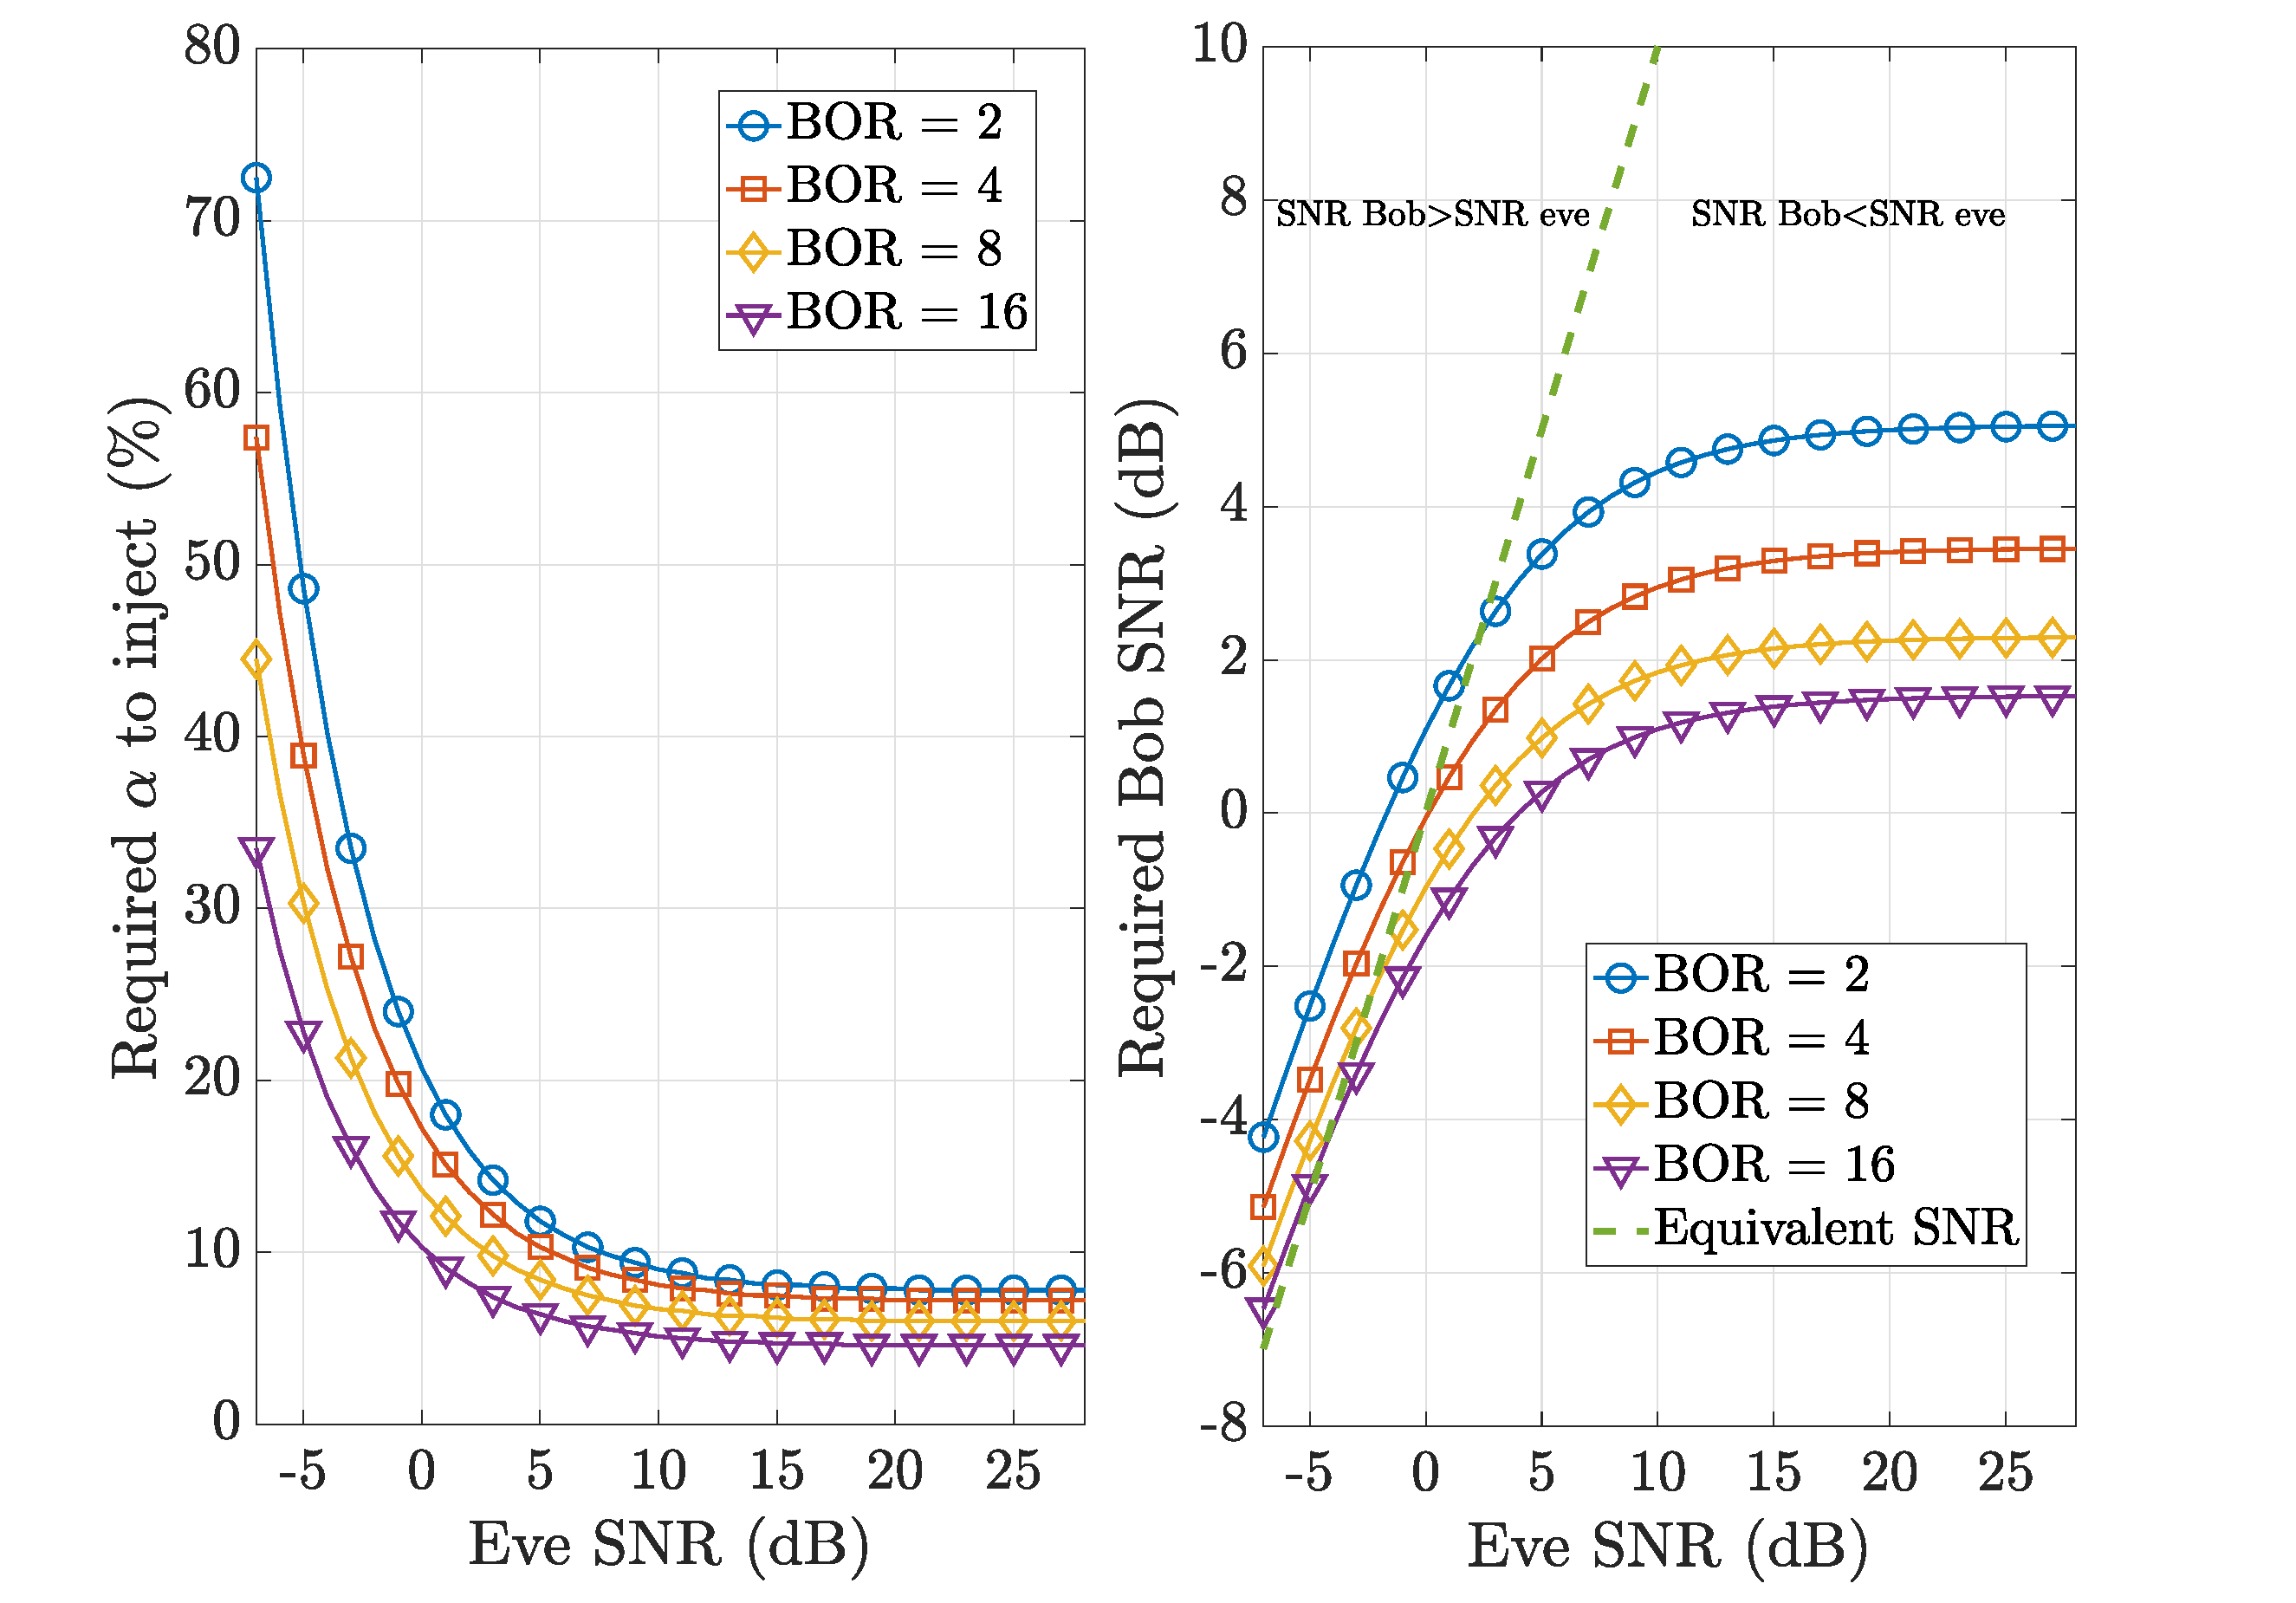
\includegraphics[width=1\linewidth]{graphs/SISO_no_corr_targettedSR_0_model2.eps}
	\caption{Targetted SR = 0 bit/channel use, matched filtering at Eve}
	\label{fig_targettedSR}
\end{figure} 



%%
\subsection{Waterfilling optimization performances}
{\color{red} Equivalent of fig13 p15 rapport + comments \\

ATTENTION: REFAIRE SIMU + LONGUE AU LABO}

\begin{figure}[h!t]
	\centering
	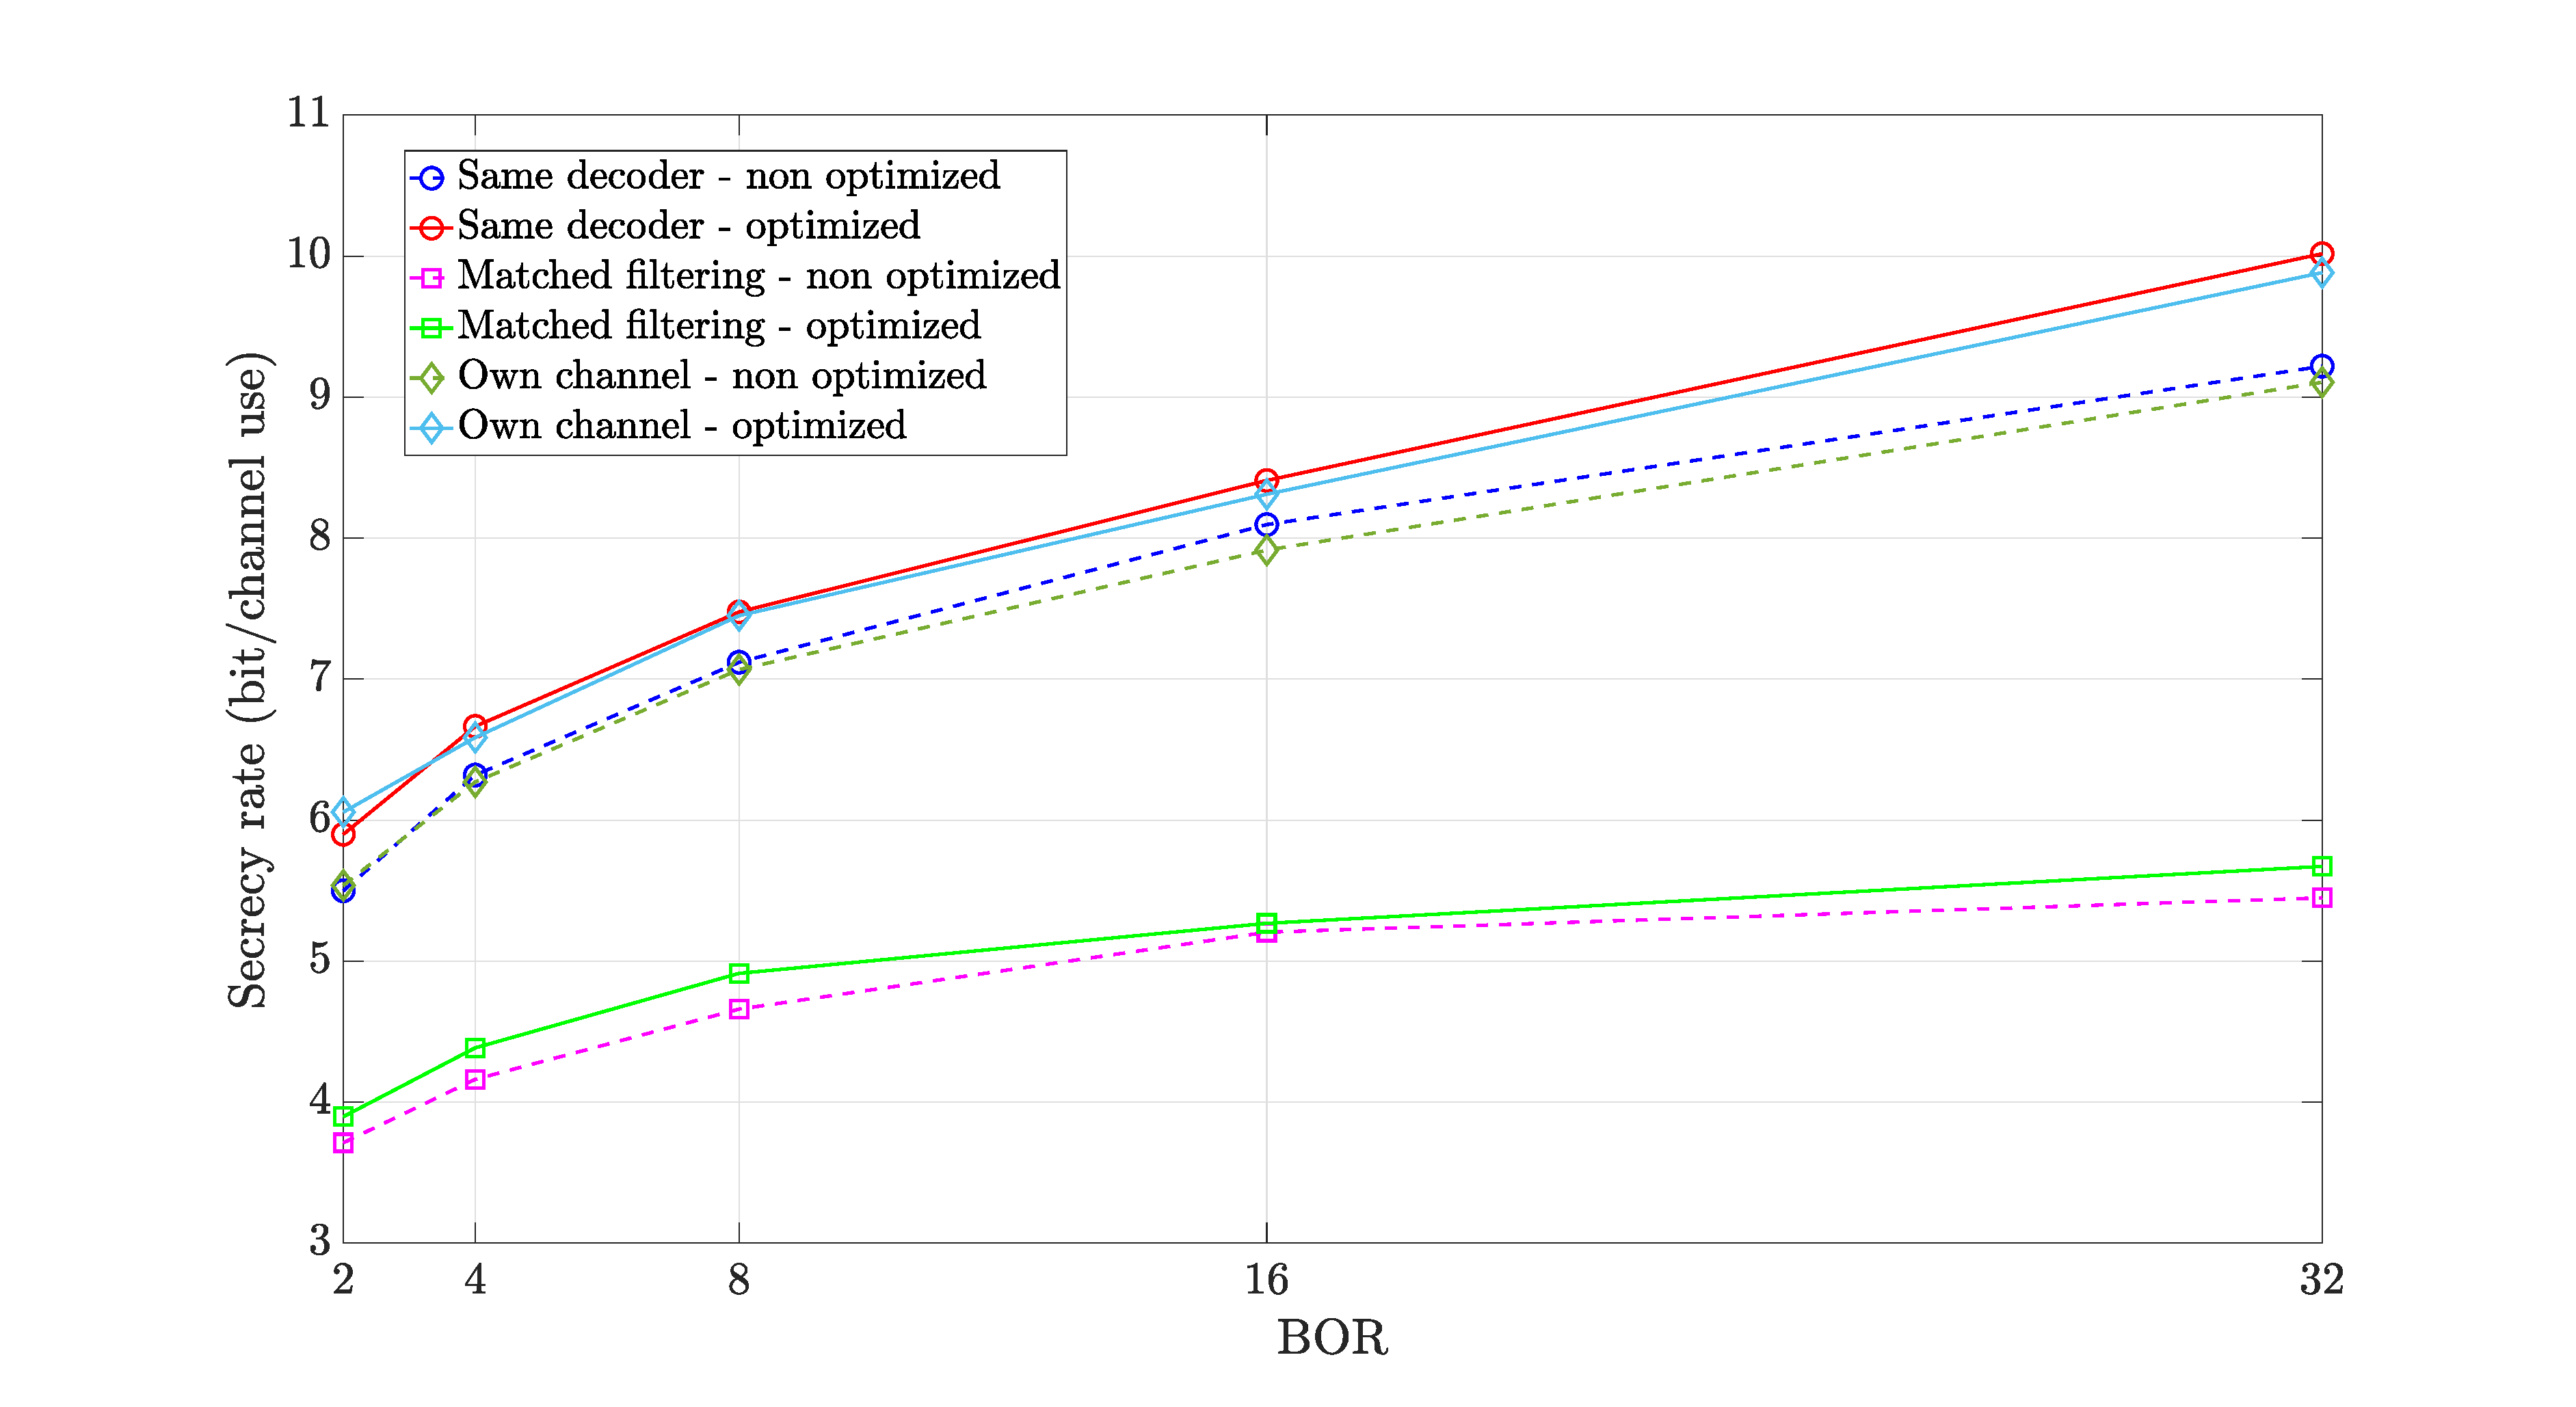
\includegraphics[width=1\linewidth]{graphs/SISO_no_corr_waterfilling.eps}
	\caption{Waterfilling optimization, $E_b/N_0 = 15$dB at Bob and Eve, BOR = 4}
	\label{fig_waterfilling_opt}
\end{figure}




%%%%%%%%%   CONCLUSONS   %%%%%%%%% 
\section{Conclusions}







%\begin{table}[!t]
% increase table row spacing, adjust to taste
%\renewcommand{\arraystretch}{1.3}
%\caption{An Example of a Table}
%\label{table_example}
%\centering
% Some packages, such as MDW tools, offer better commands for making tables
% than the plain LaTeX2e tabular which is used here.
%\begin{tabular}{|c||c|}
%\hline
%One & Two\\
%\hline
%Three & Four\\
%\hline
%\end{tabular}
%\end{table}









%%%%%%%%%   APPENDICES  %%%%%%%%% 
\appendices
\section{Derivation of.. to define}
Appendix one text goes here.





% use section* for acknowledgment
\section*{Acknowledgment}


The authors would like to thank...

\ifCLASSOPTIONcaptionsoff
  \newpage
\fi

%%%%%%%%%   BIBLIOGRAPHY   %%%%%%%%% 

\newpage
\bibliographystyle{IEEEtran}
\bibliography{biblio} 


%%%%%%%%%   BIOGRAPHY   %%%%%%%%% 
%\begin{IEEEbiography}{Michael Shell}
%Biography text here.
%\end{IEEEbiography}

% if you will not have a photo at all:
%\begin{IEEEbiographynophoto}{John Doe}
%Biography text here.
%\end{IEEEbiographynophoto}


%\begin{IEEEbiographynophoto}{Jane Doe}
%Biography text here.
%\end{IEEEbiographynophoto}


\end{document}


